\documentclass[oneside]{article}
\usepackage{ctex}
\usepackage{amsmath}
\usepackage{fontspec}
\usepackage{bm}
\usepackage{listings}
\usepackage[usenames,dvipsnames]{xcolor}

\definecolor{mygreen}{rgb}{0,0.6,0}
\definecolor{mygray}{rgb}{0.5,0.5,0.5}
\definecolor{mymauve}{rgb}{0.58,0,0.82}
\lstset{
 backgroundcolor=\color{lightgray}, 
 basicstyle = \footnotesize,       
 breakatwhitespace = false,        
 breaklines = true,                 
 captionpos = b,                    
 commentstyle = \color{mygreen}\bfseries,
 extendedchars = false,             
 frame =shadowbox, 
 framerule=0.5pt,
 keepspaces=true,
 keywordstyle=\color{blue}\bfseries, % keyword style
 language = C++,                     % the language of code
 otherkeywords={string}, 
 numbers=left, 
 numbersep=5pt,
 numberstyle=\tiny\color{mygray},
 rulecolor=\color{black},         
 showspaces=false,  
 showstringspaces=false, 
 showtabs=false,    
 stepnumber=1,         
 stringstyle=\color{mymauve},        % string literal style
 tabsize=2,          
 title=\lstname                      
}
\title{从零开始写vio}
\author{kohill}
\date{November 2019}

\usepackage{natbib}
\usepackage{graphicx}

\begin{document}
\maketitle
\section{样例代码修改}
1. 请绘制样例代码中LM阻尼因子$\mu$随着迭代变化的曲线图
\begin{figure}[htbp]
    \centering
    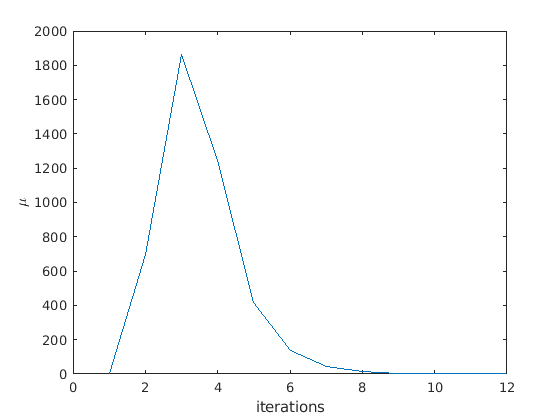
\includegraphics[width=.5\linewidth]{figures/fig1.png}    
    \caption{阻尼因子$\mu$随着迭代变化的曲线图}
\end{figure}
\clearpage
2. 将曲线函数改成 $y = ax^2 + bx + c$,请修改样例代码中残差计算,
雅克比计算等函数,完成曲线参数估计。

\begin{lstlisting}[caption={}]
    #include <iostream>
    #include <random>
    #include "backend/problem.h"
    
    using namespace myslam::backend;
    using namespace std;
    
    // 曲线模型的顶点,模板参数:优化变量维度和数据类型
    class CurveFittingVertex: public Vertex
    {
    public:
        EIGEN_MAKE_ALIGNED_OPERATOR_NEW
    
        CurveFittingVertex(): Vertex(3) {}  // abc: 三个参数, Vertex 是 3 维的
        virtual std::string TypeInfo() const { return "abc"; }
    };
    
    // 误差模型 模板参数:观测值维度,类型,连接顶点类型
    class CurveFittingEdge: public Edge
    {
    public:
        EIGEN_MAKE_ALIGNED_OPERATOR_NEW
        CurveFittingEdge( double x, double y ): Edge(1,1, std::vector<std::string>{"abc"}) {
            x_ = x;
            y_ = y;
        }
        // 计算曲线模型误差
        virtual void ComputeResidual() override
        {
            Vec3 abc = verticies_[0]->Parameters();  // 估计的参数
            residual_(0) = abc(0)*x_*x_ + abc(1)*x_ + abc(2) - y_;  // 构建残差
        }
    
        // 计算残差对变量的雅克比
        virtual void ComputeJacobians() override
        {
            Eigen::Matrix<double, 1, 3> jaco_abc;  // 误差为1维,状态量 3 个,所以是 1x3 的雅克比矩阵
            jaco_abc << x_ * x_, x_ , 1;
            jacobians_[0] = jaco_abc;
        }
        /// 返回边的类型信息
        virtual std::string TypeInfo() const override { return "CurveFittingEdge"; }
    public:
        double x_,y_;  // x 值, y 值为 _measurement
    };
    
    int main()
    {
        double a=1.0, b=2.0, c=1.0;         // 真实参数值
        int N = 1000;                          // 数据点
        double w_sigma= 1.;                 // 噪声Sigma值
    
        std::default_random_engine generator;
        std::normal_distribution<double> noise(0.,w_sigma);
    
        // 构建 problem
        Problem problem(Problem::ProblemType::GENERIC_PROBLEM);
        shared_ptr< CurveFittingVertex > vertex(new CurveFittingVertex());
    
        // 设定待估计参数 a, b, c初始值
        vertex->SetParameters(Eigen::Vector3d (0.,0.,0.));
        // 将待估计的参数加入最小二乘问题
        problem.AddVertex(vertex);
    
        // 构造 N 次观测
        for (int i = 0; i < N; ++i) {
    
            double x = i/100.;
            double n = noise(generator);
            // 观测 y
            double y = a*x*x + b*x + c + n;
    //        double y = std::exp( a*x*x + b*x + c );
    
            // 每个观测对应的残差函数
            shared_ptr< CurveFittingEdge > edge(new CurveFittingEdge(x,y));
            std::vector<std::shared_ptr<Vertex>> edge_vertex;
            edge_vertex.push_back(vertex);
            edge->SetVertex(edge_vertex);
    
            // 把这个残差添加到最小二乘问题
            problem.AddEdge(edge);
        }
    
        std::cout<<"\nTest CurveFitting start..."<<std::endl;
        /// 使用 LM 求解
        problem.Solve(300);
    
        std::cout << "-------After optimization, we got these parameters :" << std::endl;
        std::cout << vertex->Parameters().transpose() << std::endl;
        std::cout << "-------ground truth: " << std::endl;
        std::cout << "1.0,  2.0,  1.0" << std::endl;
    
        // std
        return 0;
    }
    
    
\end{lstlisting}

\begin{figure}[htbp]
    \centering
    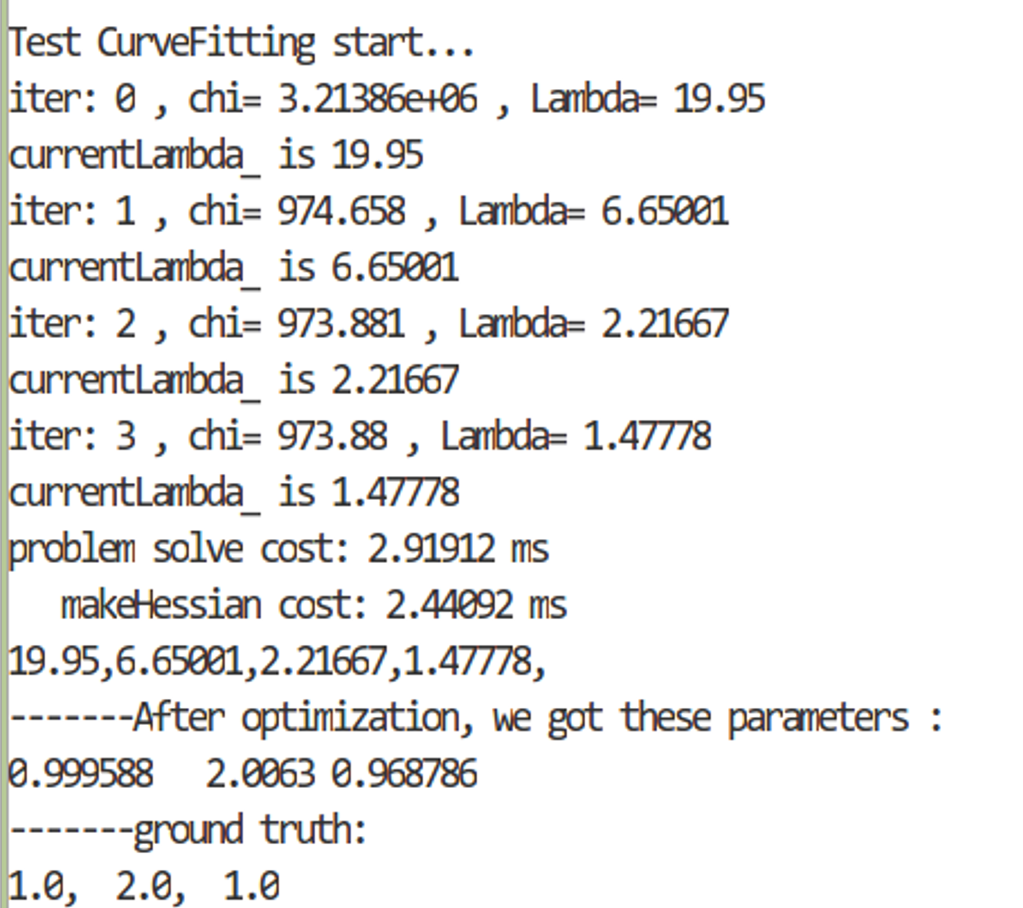
\includegraphics[width=.5\linewidth]{figures/fig2.png}    
    \caption{运行结果截图}
\end{figure}
\clearpage

\section{公式推导}
\begin{figure}[htbp]
    \centering
    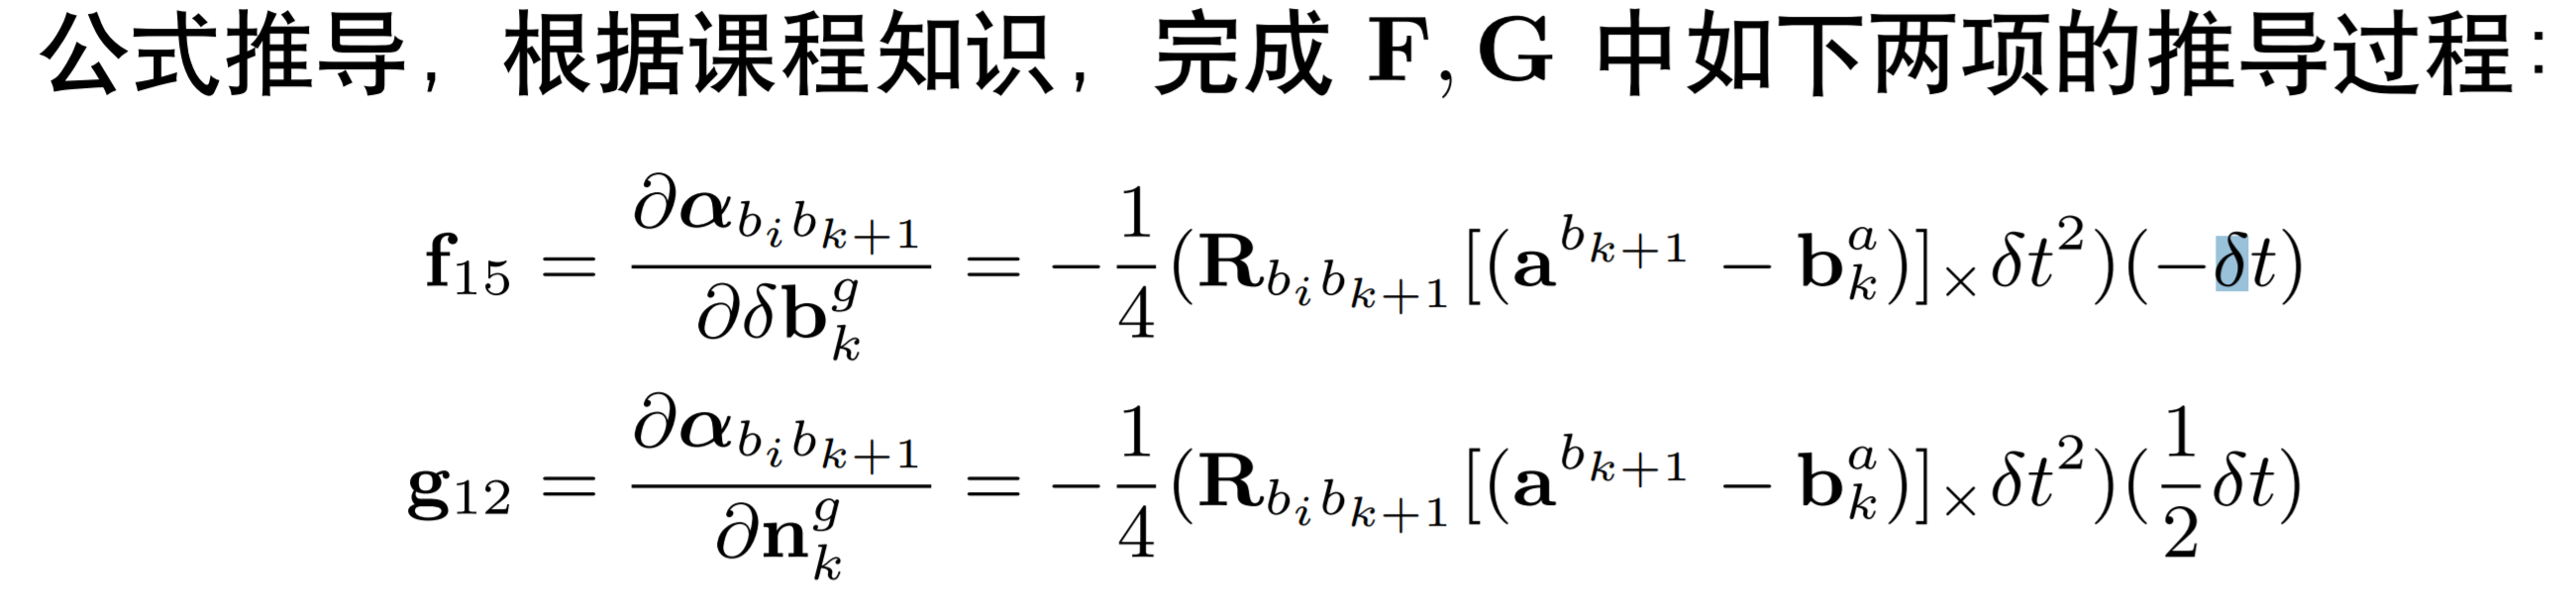
\includegraphics[width=.8\linewidth]{figures/fig3.png}    
\end{figure}
\begin{align}
    \frac{\partial \boldsymbol{\alpha}_{b_{i} b_{k+1}}}{\partial \delta \mathbf{b}_{k}^{g}}    
 &= \frac{\partial\boldsymbol{\alpha}_{b_{i} b_{k}}+\boldsymbol{\beta}_{b_{i} b_{k}} \delta t+\frac{1}{2} \mathbf{a} \delta t^{2}}{\partial \delta \mathbf{b}_{k}^{g}} \\
 &= \frac{\partial\frac{1}{2} \mathbf{a} \delta t^{2}}{\partial \delta \mathbf{b}_{k}^{g}} \\
 &= \frac{\partial\frac{1}{4}\left(\mathbf{q}_{b_{i} b_{k}}\left({\mathbf{a}}^{b_{k}}-\mathbf{b}_{k}^{a}\right)+\mathbf{q}_{b_{i} b_{k+1}}\left({\mathbf{a}}^{b_{k+1}}-\mathbf{b}_{k}^{a}\right)\right) \delta t^2}{\partial \delta \mathbf{b}_{k}^{g}} \\
 &= \frac{\partial\frac{1}{4}\left(\mathbf{q}_{b_{i} b_{k}}\left({\mathbf{a}}^{b_{k+1}}-\mathbf{b}_{k}^{a}\right)\right) \delta t^2}{\partial \delta \mathbf{b}_{k}^{g}} \\
 &= \frac{\partial\frac{1}{4}\left(\mathbf{R}_{b_{i} b_{k}}
\exp \left( \left[ \frac{1}{2}(\mathbf{\omega}^{b_k} + \mathbf{\omega}^{b_{k + 1}} - \mathbf{b}_k^g) \delta t \right]_{\mathbf{x}} \right)
 \left({\mathbf{a}}^{b_{k+1}}-\mathbf{b}_{k}^{a}\right)\right) \delta t^2}{\partial \delta \mathbf{b}_{k}^{g}} \\
\end{align} 
为了简化公式,令:
\begin{equation}
    \mathbf{O} = \left(\mathbf{R}_{b_{i} b_{k}}
    \exp \left( \left[ \frac{1}{2}(\mathbf{\omega}^{b_k} + \mathbf{\omega}^{b_{k + 1}} - \mathbf{b}_k^g) \delta t \right]_{\mathbf{x}} \right)
     \left({\mathbf{a}}^{b_{k+1}}-\mathbf{b}_{k}^{a}\right)\right)  
\end{equation}
于是:
\begin{align}
    \frac{\partial \boldsymbol{\alpha}_{b_{i} b_{k+1}}}{\partial \delta \mathbf{b}_{k}^{g}}    \\
 &= \frac{\partial\frac{1}{4}\left(\mathbf{R}_{b_{i} b_{k}}
\exp \left( \left[ \frac{1}{2}(\mathbf{\omega}^{b_k} + \mathbf{\omega}^{b_{k + 1}} - (\mathbf{b}_k^g + \delta \mathbf{b}_k^g))\delta t \right]_{\mathbf{x}}\right)
 \left({\mathbf{a}}^{b_{k+1}}-\mathbf{b}_{k}^{a}\right)-\mathbf{O} \right)   \delta t^2}{\partial \delta \mathbf{b}_{k}^{g}} \\
 &= \frac{\partial\frac{1}{4}\left(\mathbf{R}_{b_{i} b_{k}}
 \exp \left( \left[ \frac{1}{2}(\mathbf{\omega}^{b_k} + \mathbf{\omega}^{b_{k + 1}} - \mathbf{b}_k^g ) \delta t\right]_{\mathbf{x}}\right)
 \left[-\delta \mathbf{b}_k^g \delta t \right]_\mathbf{x}
  \left({\mathbf{a}}^{b_{k+1}}-\mathbf{b}_{k}^{a}\right) \right)   \delta t^2}{\partial \delta \mathbf{b}_{k}^{g}} \\
&= \frac{\partial\frac{1}{4}\left(\mathbf{R}_{b_{i} b_{k+1}}
  \left[-\delta \mathbf{b}_k^g \delta t \right]_\mathbf{x}
   \left({\mathbf{a}}^{b_{k+1}}-\mathbf{b}_{k}^{a}\right) \right)   \delta t^2}{\partial \delta \mathbf{b}_{k}^{g}}  \\
&= \frac{\partial\frac{1}{4}\left(\mathbf{R}_{b_{i} b_{k+1}}
   \left[ \left({\mathbf{a}}^{b_{k+1}}-\mathbf{b}_{k}^{a}\right) \right]_\mathbf{x}
     \right)   \delta t^2}{\partial \delta \mathbf{b}_{k}^{g}}    
    \delta \mathbf{b}_k^g \delta t \\
&= \partial\frac{1}{4}\left(\mathbf{R}_{b_{i} b_{k+1}}
    \left[ \left({\mathbf{a}}^{b_{k+1}}-\mathbf{b}_{k}^{a}\right) \right]_\mathbf{x}
      \right)   \delta t^2  \delta t  \\
&=-\frac{1}{4}\left(\mathbf{R}_{b_{i} b_{k+1}}\left[\left(\mathbf{a}^{b_{k+1}}-\mathbf{b}_{k}^{a}\right)\right]_{\mathbf{x}} \delta t^{2}\right)(-\delta t)
\end{align} 
因此PPT的f15得证。
% \begin{align}
%  \frac{\partial\frac{1}{4}\left(\mathbf{q}_{b_{i} b_{k}}\left({\mathbf{a}}^{b_{k}}-\mathbf{b}_{k}^{a}\right)+\mathbf{q}_{b_{i} b_{k+1}}\left({\mathbf{a}}^{b_{k+1}}-\mathbf{b}_{k}^{a}\right)\right)}{\partial \delta \mathbf{b}_{k}^{g}} 
%  &= \frac{\partial\frac{1}{4}\left(\mathbf{q}_{b_{i} b_{k}} \otimes\left[\begin{array}{c}{1} \\ {\frac{1}{2} \omega \delta t}\end{array}\right]\left({\mathbf{a}}^{b_{k+1}}-\mathbf{b}_{k}^{a}\right)\right)}{\partial \delta \mathbf{b}_{k}^{g}} \\
%  &= \frac{\partial\frac{1}{4}\left(\mathbf{q}_{b_{i} b_{k}} \otimes\left[\begin{array}{c}{1} \\ {\frac{1}{2} \left(\frac{1}{2}\left(\omega^{b_{k}}+\omega^{b_{k+1}}\right)-\mathbf{b}_{k}^{g}\right) \delta t}\end{array}\right]\left({\mathbf{a}}^{b_{k+1}}-\mathbf{b}_{k}^{a}\right)\right)}{\partial \delta \mathbf{b}_{k}^{g}} 
% \end{align}
\section{证明}
证明下面的结论

\begin{figure}[h]
    \centering
    
\includegraphics[width=.8\linewidth]{figures/fig4.png}    
\end{figure}

即证:$\Delta \mathbf{x}_{\operatorname{lm}}=-\sum_{j=1}^{n} \frac{\mathbf{v}_{j}^{\top} \mathbf{F}^{\prime \top}}{\lambda_{j}+\mu} \mathbf{v}_{j}$是式\ref{equa:normal_equations}的解。
\begin{equation}
    (\mathbf{J}^\top\mathbf{J} + \mu \mathbf{I}) \Delta \mathbf{x}_{\operatorname{lm}} = - \mathbf{J} ^T  \mathbf{f}
    \label{equa:normal_equations}
\end{equation}
将:$\Delta \mathbf{x}_{\operatorname{lm}}=-\sum_{j=1}^{n} \frac{\mathbf{v}_{j}^{\top} \mathbf{F}^{\prime \top}}{\lambda_{j}+\mu} \mathbf{v}_{j}$代入:
\begin{equation}
    \sum_{j=1}^{n}(\mathbf{J}^T\mathbf{J} + \mu \mathbf{I})  \frac{\mathbf{v}_{j}^{\top} \mathbf{F}^{\prime \top}}{\lambda_{j}+\mu} \mathbf{v}_{j} = \mathbf{J} ^\top  \mathbf{f}
\end{equation}
考虑到$\mathbf{J}^T\mathbf{J} + \mu \mathbf{I}$的特征值为$\lambda_{j}+\mu$:
\begin{equation}
    \sum_{j=1}^{n} \mathbf{v}_{j}^{\top} \mathbf{F}^{\prime \top} \mathbf{v}_{j} = \mathbf{J} ^\top  \mathbf{f} 
\end{equation}
也即:

\begin{align}
    % \mathbf{J} ^ \top \mathbf{J}
    \sum_{j=1}^{n} \mathbf{v}_{j}^{\top} \mathbf{J} ^ \top  \mathbf{f}  \mathbf{v}_{j} &= \mathbf{J} ^\top  \mathbf{f} \\
    \sum_{j=1}^{n} \frac{1}{\lambda_{j} ^2}\mathbf{v}_{j}^{\top} \mathbf{J} ^ \top \mathbf{J} \mathbf{J} ^ \top  \mathbf{f}  \mathbf{J} ^ \top \mathbf{J} \mathbf{v}_{j} &= \mathbf{J} ^\top  \mathbf{f}
\end{align}
注意到其中有个常数项,将它交换位置:
\begin{equation}
    \sum_{j=1}^{n} \frac{1}{\lambda_{j} ^2}  \mathbf{J} ^ \top \mathbf{J} \mathbf{v}_{j} \mathbf{v}_{j}^{\top} \mathbf{J} ^ \top \mathbf{J} \mathbf{J} ^ \top  \mathbf{f} = \mathbf{J} ^\top  \mathbf{f}     
\end{equation}
将$\mathbf{J}^{\top} \mathbf{J}=\mathbf{V} \bm{\mathbf{\Lambda}} \mathbf{V}^{\top}$带入:
\begin{equation}
    \sum_{j=1}^{n} \frac{1}{\lambda_{j} ^2}  \mathbf{V} \bm{\mathbf{\Lambda}} \mathbf{V}^{\top} \mathbf{v}_{j} \mathbf{v}_{j}^{\top} \mathbf{V} \bm{\mathbf{\Lambda}} \mathbf{V}^{\top} \mathbf{J} ^ \top  \mathbf{f} = \mathbf{J} ^\top  \mathbf{f}     
    \label{equa:prov_pre}
\end{equation}
考虑特征向量之间线性无关,且$\mathbf{V}$为正交矩阵,$\bm{\mathbf{\Lambda}}$为对角矩阵,可得:
\begin{equation}
    \sum_{j=1}^{n} \frac{1}{\lambda_{j} ^2}  \mathbf{V} \bm{\mathbf{\Lambda}} \mathbf{V}^{\top} \mathbf{v}_{j} \mathbf{v}_{j}^{\top} \mathbf{V} \bm{\mathbf{\Lambda}} \mathbf{V}^{\top} = \mathbf{I} 
\end{equation}
因此式\ref{equa:prov_pre}显然成立,原式得证。
\end{document}

